\chapter{Introduction}
\label{c:intro}

% \section{Motivation}
% \label{section:motivation}
% Algriculture is the key role for human history~\cite{agri-wiki}. Increasing of food productivity allows people to develop technology and civilization. In Taiwan 1945, after regime transferred to Government of Republic of China, ratio of farming land even reached 34\% of Taiwan's land use~\cite{agri-land}. Owing to mechanize technology from modern society, the productivity of farming has a huge growth by synthetic fertilizers, pesticides and automation. 

% \begin{figure}[!h]
%     \centering
%     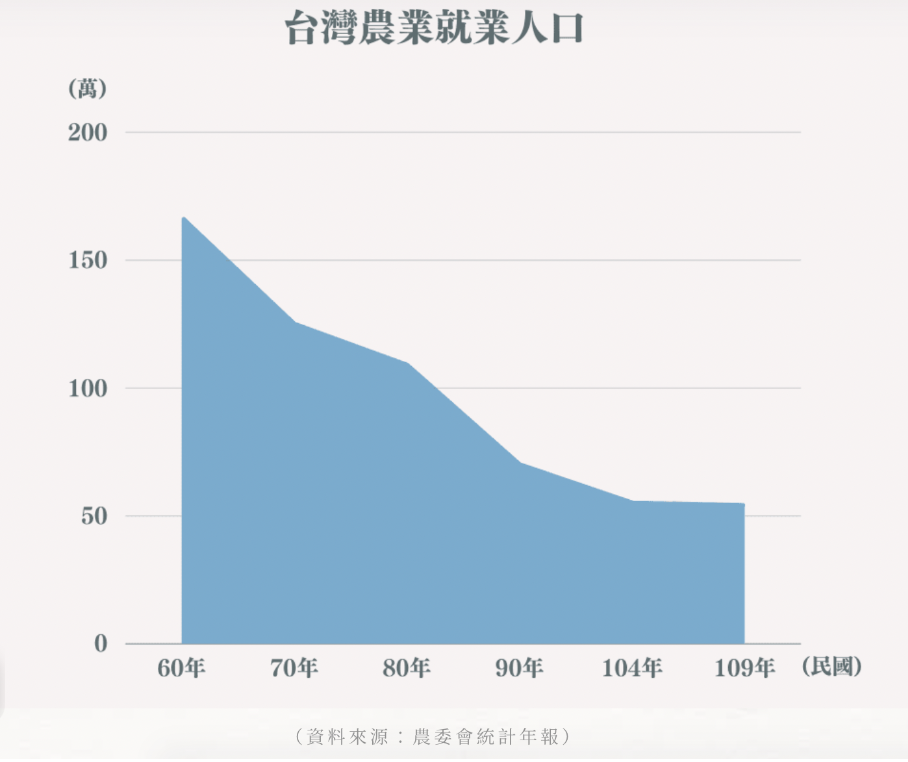
\includegraphics[width=\textwidth]{figsrc/agri_population.png}
%     \caption{The decreasing of farming population.\label{fig:population}}
% \end{figure}

% 講農業
% In chapter 1, we will explain why we need video recording system.


One of the most critical improvement of technology human beings have ever made must be the domestication of plants during the agricultural revolution 8-12,000 years ago at multiple sites around the world~\cite{agri-wiki}~\cite{agri-history}. These innovation of new food resource created civilizations and other new technology by steady and predictable supply of calories through human work. The human population have drastically increased to 7.97 billion as of September 2022 according to the most recent United Nations estimates elaborated by Worldometer~\cite{argi-pop}. This has been made possible by an efficient and productive agricultural basis~\cite{agri-pop2}.
% 講畜牧業
Another critical invention is livestock farming. Domesticated animals are raised in an agricultural field. It can offer labor and produce food resuorce such as meat and milk~\cite{agri-stock}. Overall, livestock provides 33\% percent of the protein for human diet~\cite{agri-stock2}.
% 講工業農業->講農業畜牧業遇到的問題(quality and diseases)
Thanks to industrial revolution that happened between the 17th century and the mid-19th century. Human took advantage of mechanize technology, such as using pesticides to reduce damage of pests, applying synthetic fertilizer to supply plant nutrients and mechanised device greatly increasing crop worker productivity. Although industrial revolution helps a lot, we still face some problems. Crop farming is threatened by infectious diseases and damage of pests due to globalization combined with climate change~\cite{crop-fail}. Diseases occured in either stock or crop farming that need to be improved. As the human population becomes larger and larger. Productivity of food need to further increase to provide even more calories and nutrition. In fish farming, it is costly and tiring operation that require a lot of man power, more than 67\% of farm costs go to the workforce~\cite{fish-labour}. We need some more advanced technology to solve the problems for diseases and automation.

% AI iot 
When it comes to modern technology, we will mention about Artificial Intelligence(AI) and Internet of Things(IOT). We call farm which combine with AI and IOT as smart farm. Smart farm has tremendous potential to solve the problem whilch we mention above based on AI computer vision and communications via internet. Previous research about dragonfruit~\cite{agri-ai} design a precise agriculture system for classifying different ripeness of dragonfruits, then transmit the prediction result to refitted fruit gravity classifier which can grade dragonfruits automatically. It is more complex in stock farming. For reognition or classification of crop, it uses photo data to train AI model. Although there are also some tasks that use photo as trianing set, behaviour analysis soon becomes problem. Because behaviour is the range of actions and mannerisms. In other words, it is hard to be recognized by a single photo. Thus, continuous motion data, video data, is considered better than single static data in this case. For example, in ~\cite{fish-paper}, It used video files to extract the identification of fish trajectories and analyze their behaviors through trajectories. In ~\cite{cow-paper}, video data were used for the real-time capture of rutting behavior and hoof or back characteristics. ~\cite{hens-paper} classified the behavior of a single laying hen. Allow user to identify three different types of individual behavior (standing, walking, and scratching).

In this thesis, we propose a automatic cloud based recording system implemented in Smart Farming Platform~\cite{agri-web}. Smart Farming Platform is a platform built by National Tsing Hua University High Speed Network Lab. This recording system has multiple services that are capable of executing different type of collecting data tasks. For example, our system provide user to manually start record task by clicking a button. Also, it can let user schedule its own timing to trigger record tasks. At last, user can register some event which is critical. When the event occurs, system will dynamically  start record process. All of the services is based on the basic function of Smart Farming Platform. It is easy for user to use for collecting video data empowered by automatical system. It is flexible, storage limitless, easy to maintain. Most of the system is implemented in AWS cloud service~\cite{aws}. In chapter 2, we will introduce some related work about recording system. Chapter 3 will explain the detail of the system by each user case. Chapter 4 will show the result of the system including demonstration of the various user cases and analyze the performance of the system. Chapter 5 will make conclusion and show the future work.

% 講現在是怎麼解決的
% 但畜牧業遇到什麼問題(資料收集困難...等)
% 我們提出的東西

% In Taiwan, although we also took advantage of mechanize technology, we still encountered some problem such as potential dropping of food productivity due to lack of will from young people to join agriculture. Most of them are more willing to seek for higher paid job rather than being a farmer. This lead to the distribution of farming population became older and older and decreasing of farming population~\cite{agri-population}. Fig.~\ref{fig:population} shown the recent trend of farming population. To solve the issue, society and government tried to introduce Industry 4.0 technology such as high concentration of LED, robotics, engineering, and data processing firms~\cite{agri-import-tech}. 



% 詳細介紹平台功能
% In this platform, previous research collected various data from experimental field such as crop photo, pH and moisture of soil by different type of sensors and IP Cam, 360 Degree high speed camera ~\cite{IPcam}. In this thesis, we will mainly focus on the function related to IP cam.

% \begin{figure}[!htb]
%     \centering
%     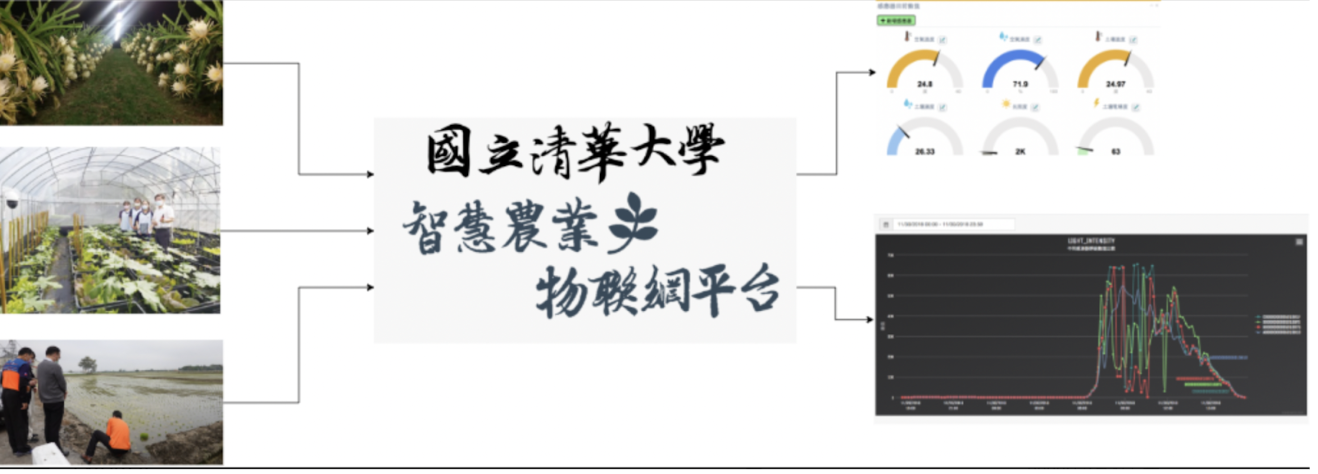
\includegraphics[width=\textwidth]{figsrc/IOT_plat.png}
%     \caption{Agriculture AIOT platform.\label{fig:IOT_plat}}
% \end{figure}

% % sensor: 用什麼收集資料,土壤bla bla bla。
% % 農業日誌

% % IP cam
% For AI training, they implemented streaming module that can see live streaming from farm or other experimental field and store photo to AWS S3~\cite{aws-s3}. As showned in fig.~\ref{fig:IPcamRoughDataFlow}, They used IP cam to push stream to web page for user to supervise on site remotely and preset to collect data periodically(i.e. Set specific times for camera to take picture repeatly). We will show further detail about IPcam in Ch3. 
% \begin{figure}[!htb]
%     \centering
%     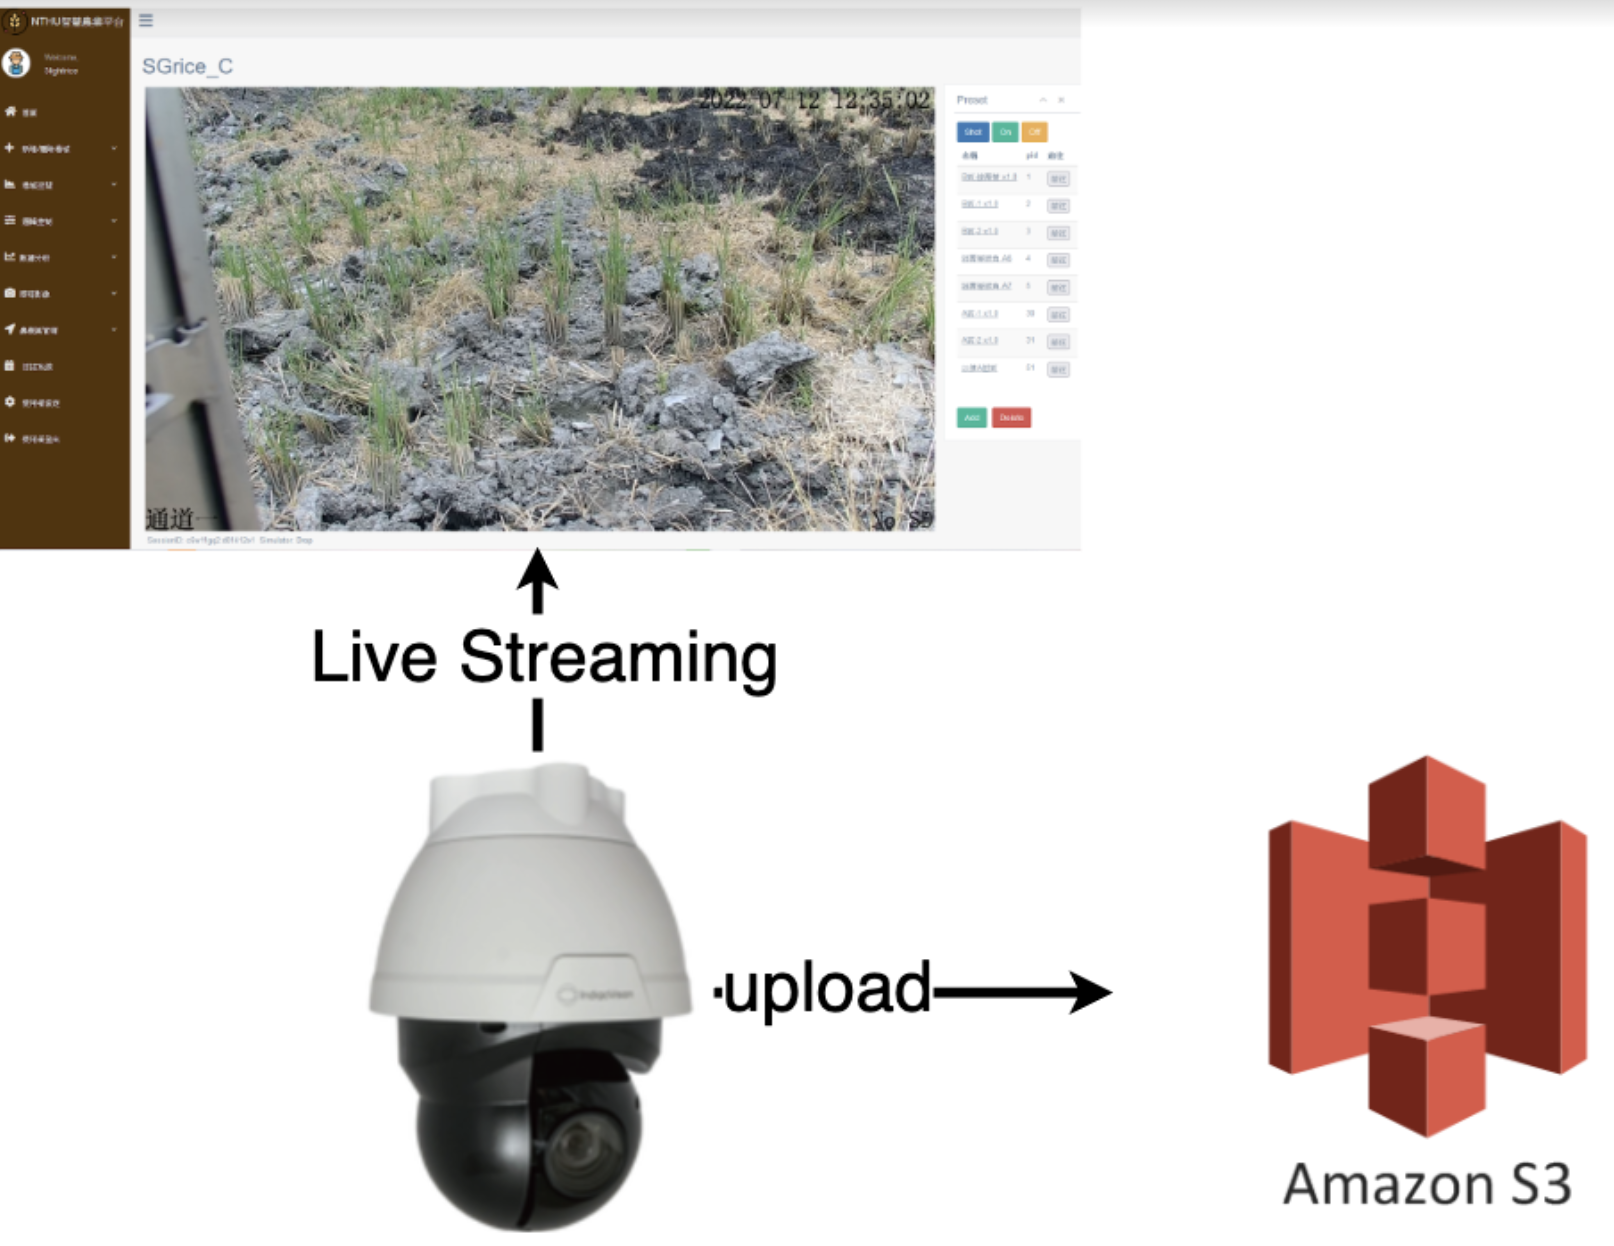
\includegraphics[width=\textwidth]{figsrc/IPcamRoughDataFlow.png}
%     \caption{IP cam push stream to web page and store photo to S3.\label{fig:IPcamRoughDataFlow}}
% \end{figure}

% % 可改進的地方
% Previous research had established a variety of function to asist agriculture. But it still had some issues that could be improved. Below, we focused on the issues around IP camera.

% First, stability of IP cam control. As shown in Fig.~\ref{fig:IPcam-dataflow}, we had to send request to camera if we wanted to rotate camera to specific angle or did other operations. It appeared that camera failed to recieve command at ratio of 23\% (e.g. If someone wanted to send rotation command to camera, camera would have 23\% probability failed to receive.). Thus, the camera control UX for user could be further improved.

% \begin{figure}[!htb]
%     \centering
%     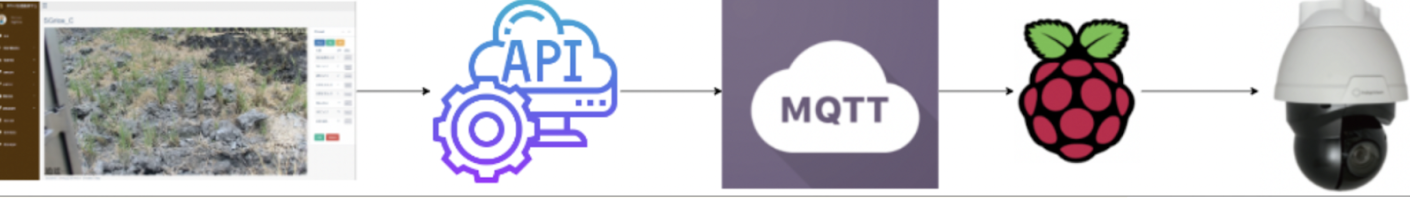
\includegraphics[width=\textwidth]{figsrc/IPcam-dataflow.png}
%     \caption{Data flow of request from web page to camera.\label{fig:IPcam-dataflow}}
% \end{figure}

% Second, scalability of edge device. As we mentioned above, we sent request to camera if we wanted to do any operaion. The data flow between web page and camera were shown in Fig.~\ref{fig:IPcam-dataflow}. There were five components involved: Front-end server served as web page sent API request to API server; API server recieved request and sent MQTT message to MQTT broker [-x-]; MQTT broker transmitted message to raspberry PI~\cite{PI-intro}; At last, raspberry PI commanded camera to execute locally. The problem of controling camera by PI was that the deployed function for controlling camera was only capable of commanding single device. In other word, it had to deploy multiple identical function to control more than one camera as shown in Fig.~\ref{fig:PI-scalability-improvement}. This would cause redundant resource wasting and difficuty of maintaining system.

% \begin{figure}[!htb]
%     \centering
%     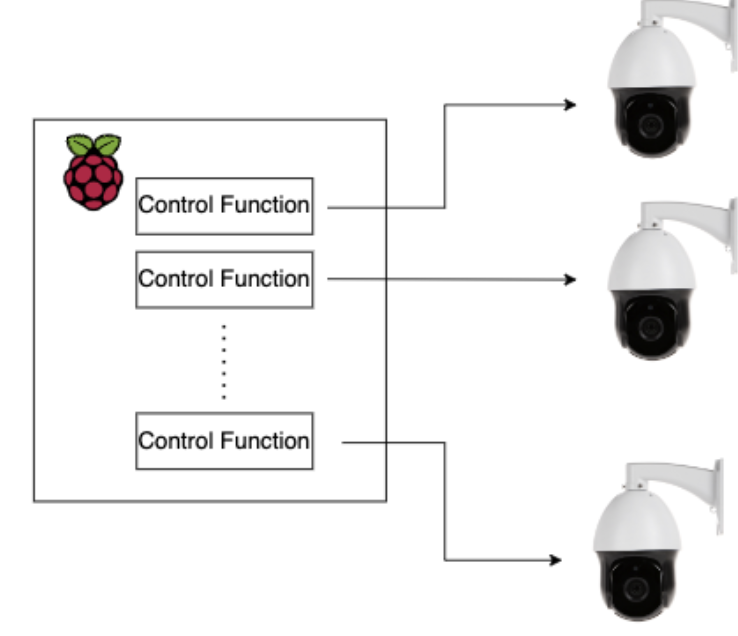
\includegraphics[width=\textwidth]{figsrc/PI-scalability-improvement.png}
%     \caption{Issue of scalability for PI.\label{fig:PI-scalability-improvement}}
% \end{figure}

% Third, data losing. One of the main task of camera was to collect data continuously for other researchers used as AI training. The problem about data collection is due to various external factors such as power failure, rainstorm, long-term sun exposure etc.. Edge devices located in experimental field would malfunction result from the factors mentioned before. Current system didn't have mechanism to detect edge devices failure then notified researchers to repair it in time. This had risk of losing large amount of data without noticed. 

% Fourth, video colleciton. Current system supported photo collection as data source for Conputer Vision AI model. But in case of model training that required video, manually recording or time scheduling, it wasn't available for researchers. For instance, fig.~\ref{fig:aqua-live-stream} was fish farm of Aquaculture Research Lab in HuaLian~\cite{aqua-intro}. For research related to fish shoal, we needed video instead of photo to analyze data such as vitality of fish.

% \begin{figure}[!htb]
%     \centering
%     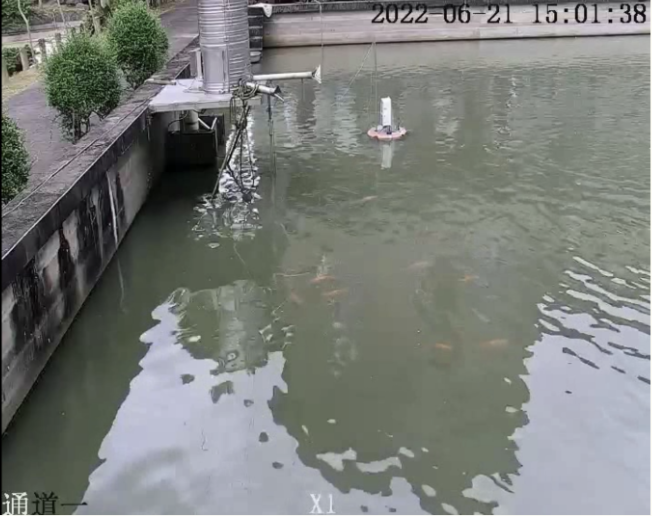
\includegraphics[width=\textwidth]{figsrc/aqua-live-stream.png}
%     \caption{Live image in Aquaculture Research Lab in HuaLian.\label{fig:aqua-live-stream}}
% \end{figure}

% In this thesis, we propose various optimization of system issues around IP cam such as stability of IP cam, scalability of edge device and data losing. Also we design and implenemt video collector from scratch to meet the requirement for video-type data. In Chapter 2, we will introduce the related technology we used in the following chapters. In Chapter 3, we will describe the detail of camera related optimization of system and show how we enhance stability, scalability and reduce data losing damage of the system. In Chapter 4, we show the whole procedure of how we build the video collector from scratch. From requirement analysis, prototyping to system development. Include details of structure in every components and critical cases. In Chapter 5, we demonstrate the correctness of the video collector including handling critical cases. In Chapter 6, the summary and future work of proposed solutions and system of this thesis.

%================

% In this platform, we can store variety of data(e.g. crop images, soil moisture and PH etc.) on platform by corresponding sensor or IP Cam. Utilize data for various purpose such as making diagram for expert to do systematic analysis or using as data set for AI model training. But it still have some issues can be improved. For instance: stability, scalability, system failure notification. At last, lack of video collecting solution to fit the analysis that require video data. In this thesis, We propose the solution for system optimization and implementation for video collector.

% 如果需要參考模板,就把下面這些uncomment
% \begin{figure}[!htb]
%     \centering
%     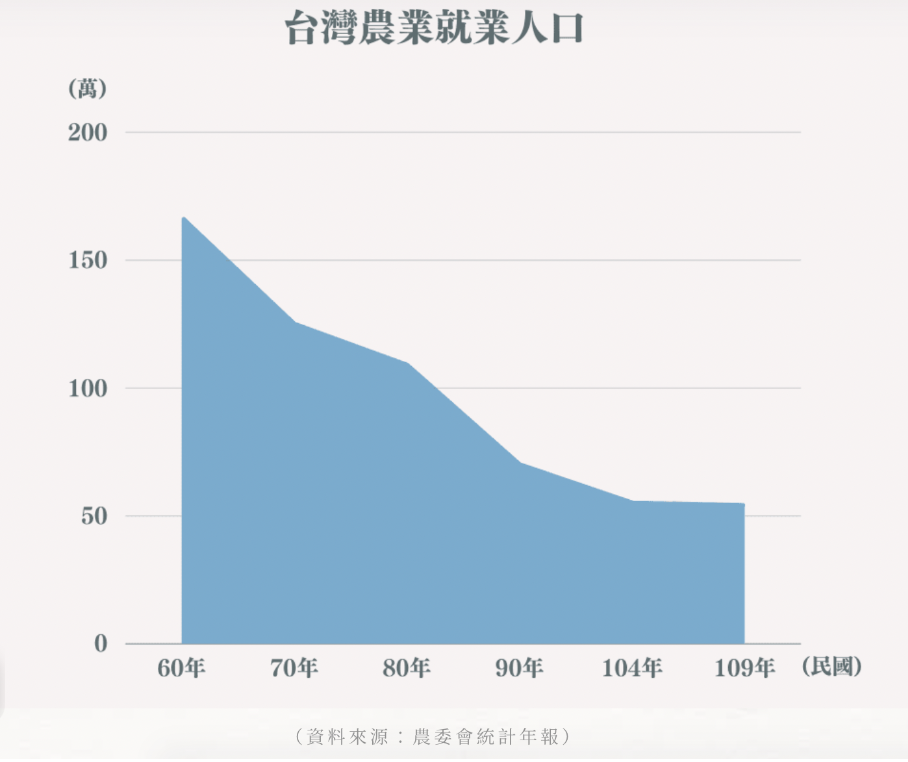
\includegraphics[width=\textwidth]{figsrc/agri_population.png}
%     % \caption{A diagram showing how divide and conquer works.\label{fig:DnC}}
% \end{figure}
% \section{Goal}
% \label{section:goal}
% Design a software that converts a score image (.png / .jpeg / .bmp / .pdf) into its symbolic representation encoded in a format that is readable by a computer such as MusicXML.

% \section{Divide and Conquer}
% \subsection{Definition}
% \label{section:divide-and-conquer}

% Fig.~\ref{fig:DnC} shows the concepts of \emph{divide and conquer} (D\&C). D\&C is an algorithm design paradigm that breaks a complex problem into a couple of relatively simple subproblems, to \emph{divide}, then solves them respectively, to \emph{conquer}. Before conquering, the problem will be divided recursively until it is simple enough to be processed. Finally, the solutions to the subproblems will be merged as those to the original problem.



% \subsection{Main Contribution of This Dissertation}
% \label{subsec:advantages}

% \subsubsection{Reducing the Difficulty of Problems}

% Due to characteristics of D\&C, all problems that can be accurately split are expected to be solved. For this dissertation, particularly, if the function detecting staves is reliable, then we can analyze arbitrarily complicated scores.

% \subsubsection{Independence of Subproblems}

% Typically, a score contains something useless for recognition such as the metadata of the song, lyrics, and even printed defects. By partitioning the original images into subimages where each contains only one staff, the amount of noisy information can be reduced and interference between staves is eliminated. Therefore, the detection tasks are independent between different staves.

% \subsubsection{Parallelism}

% Nowadays, a processor usually has multiple cores, and lots of computational tasks are implemented to be executed with parallel programs. In D\&C algorithm, the functions solving split subproblems are identically designed. With high independence and similar operations between subproblems, it is a good strategy to process them simultaneously. In other word, the original problem is suitable to be solved with \emph{SIMD (Single-Instruction-Multiple-Data)} parallel programs.
